\documentclass[main.tex]{subfiles}
\begin{document}

\chapter{The Karlin--Rubin Theorem and UMP Tests}\label{ch:karlin-rubin}

The Neyman--Pearson\index{neyman pearson lemma@Neyman--Pearson lemma} lemma gives the optimal test for two \emph{simple} hypotheses. In real problems, however, the alternative is almost always composite, as in ``the new drug is more effective'' ($\theta>\theta_0$). A test that is most powerful simultaneously at every point of a composite alternative is called a \emph{uniformly most powerful\index{uniformly most powerful ump test@uniformly most powerful (UMP) test}} (UMP) test. The existence of such a test is a strong requirement; the Karlin--Rubin\index{karlin rubin theorem@Karlin--Rubin theorem} theorem shows that it is met for one-sided hypotheses in families whose likelihood ratio\index{likelihood ratio@likelihood ratio} is monotone in a statistic. In this chapter we also discuss why no UMP test exists in two-sided problems and how the constraint of unbiasedness fills this gap.

\section{Definitions}

\begin{definition}[Uniformly Most Powerful (UMP) Test]\index{uniformly most powerful ump test@uniformly most powerful (UMP) test|textbf}
A level-$\alpha$ test $\phi^*$ is called a level-$\alpha$ \emph{UMP test} of $H_0:\theta\in\Theta_0$ against $H_1:\theta\in\Theta_1$ if $\beta_{\phi^*}(\theta)\ge\beta_\phi(\theta)$ for every level-$\alpha$ test $\phi$ and \emph{every} $\theta\in\Theta_1$.
\end{definition}

\begin{definition}[Monotone Likelihood Ratio (MLR)]\label{def:mlr}\index{monotone likelihood ratio mlr@monotone likelihood ratio (MLR)|textbf}
Let $\Theta\subseteq\R$. If for every $\theta_1<\theta_2$ the likelihood ratio\index{likelihood ratio@likelihood ratio}
\[
\frac{L(\theta_2;\x)}{L(\theta_1;\x)}
\]
(on $\{\x: L(\theta_1;\x)>0 \text{ or } L(\theta_2;\x)>0\}$) is a \emph{non-decreasing} function of a statistic $T(\x)$, the family is said to have a \emph{monotone likelihood ratio} (MLR) in $T$. If the ratio is a non-increasing function of $T$, the family has MLR in $-T$.
\end{definition}

\begin{definition}[Unbiased Test]
If $\sup_{\theta\in\Theta_0}\beta_\phi(\theta)\le\alpha\le\inf_{\theta\in\Theta_1}\beta_\phi(\theta)$, then $\phi$ is an \emph{unbiased} level-$\alpha$ test: it rejects $H_0$ more often when it is false than when it is true. A test that is UMP among unbiased tests\index{unbiased test@unbiased test} is called a \emph{UMPU\index{umpu test@UMPU test}} test.
\end{definition}

\section{Main Theorems and Proofs}

\begin{proposition}[MLR in the Exponential Family]\label{prop:ustel-mlr}\index{monotone likelihood ratio mlr@monotone likelihood ratio (MLR)}
Let $f(x;\theta)=h(x)c(\theta)\exp\{w(\theta)t(x)\}$ be a one-parameter exponential family\index{exponential family@exponential family} and $T=\sum t(X_i)$. If $w$ is non-decreasing the family has MLR in $T$; if it is non-increasing, in $-T$.
\end{proposition}
\begin{proof}
For $\theta_1<\theta_2$, $\frac{L(\theta_2)}{L(\theta_1)}=\Big(\frac{c(\theta_2)}{c(\theta_1)}\Big)^n\exp\{[w(\theta_2)-w(\theta_1)]T\}$; the coefficient in the exponent is $\ge0$ if $w$ is non-decreasing.
\end{proof}

\begin{theorem}[Karlin--Rubin Theorem \cite{karlin-rubin56}]\label{thm:karlin-rubin}\index{karlin rubin theorem@Karlin--Rubin theorem}
Let the family have MLR in $T$, and test $H_0: \theta \le \theta_0$ against $H_1: \theta > \theta_0$. For $\alpha\in(0,1)$ the test
\[
\phi^*(\x)=\begin{cases}1,& T(\x)>c\\ \gamma, & T(\x)=c\\ 0, & T(\x)<c\end{cases},\qquad \E_{\theta_0}[\phi^*]=\alpha
\]
(for continuous $T$, briefly ``reject if $T(\X)>c$'') is a UMP level-$\alpha$ test. Moreover the power function\index{power function@power function} $\beta_{\phi^*}(\theta)$ is non-decreasing, and strictly increasing at every point where $\beta_{\phi^*}(\theta)<1$.

If the family has MLR in $-T$ (or if the hypotheses are $H_0:\theta\ge\theta_0$, $H_1:\theta<\theta_0$), the inequalities are reversed: ``reject if $T(\X)<c$''.
\end{theorem}
\begin{proof}
\emph{Step 1 (MP against each simple alternative).} Fix $\theta_1>\theta_0$. By MLR, $L(\theta_1)/L(\theta_0)=g(T)$ with $g$ non-decreasing. Taking $k=g(c)$, $\{T>c\}\subseteq\{g(T)\ge k\}$ and $\{g(T)>k\}\subseteq\{T>c\}$ or $\{T\ge c\}$; hence $\phi^*$ has the Neyman--Pearson\index{neyman pearson lemma@Neyman--Pearson lemma} form (Theorem~\ref{thm:neyman-pearson}(1)) and is MP at level $\alpha$ for $\theta_0$ against $\theta_1$. The crucial point: $c$ and $\gamma$ are determined solely by the condition $\E_{\theta_0}\phi^*=\alpha$ and \emph{do not depend on $\theta_1$}.

\emph{Step 2 (the power is monotone).} Take $\theta'<\theta''$. By the reasoning of Step~1, $\phi^*$ is MP at level $\beta_{\phi^*}(\theta')$ for $\theta'$ against $\theta''$. By Corollary~\ref{cor:mp-yansiz}, $\beta_{\phi^*}(\theta'')\ge\beta_{\phi^*}(\theta')$.

\emph{Step 3 (level $\alpha$).} By Step~2, $\sup_{\theta\le\theta_0}\beta_{\phi^*}(\theta)=\beta_{\phi^*}(\theta_0)=\alpha$.

\emph{Step 4 (UMP).} Let $\phi$ be any level-$\alpha$ test for the composite $H_0$. In particular $\beta_\phi(\theta_0)\le\alpha$, i.e.\ $\phi$ also has level $\alpha$ for the simple $H_0:\theta=\theta_0$. By Step~1, $\beta_{\phi^*}(\theta_1)\ge\beta_\phi(\theta_1)$ for every $\theta_1>\theta_0$.
\end{proof}

\begin{proposition}[No UMP Test in the Two-Sided Problem]\label{prop:iki-tarafli}\index{uniformly most powerful ump test@uniformly most powerful (UMP) test}
Let $X_i\iid\Normal(\mu,\sigma^2)$ with $\sigma$ known, $H_0:\mu=\mu_0$, $H_1:\mu\neq\mu_0$, $\alpha\in(0,1)$. There is no UMP test for this problem.
\end{proposition}
\begin{proof}
If a UMP $\phi$ existed, it would have to be MP for every $\mu_1>\mu_0$; by the necessity part of Neyman--Pearson (Theorem~\ref{thm:neyman-pearson}(3)), $\phi=\I\{\bar X>\mu_0+z_\alpha\sigma/\sqrt n\}$ a.e. Likewise it would have to be MP for every $\mu_1<\mu_0$, i.e.\ $\phi=\I\{\bar X<\mu_0-z_\alpha\sigma/\sqrt n\}$ a.e. These two tests differ on a set of positive probability; contradiction.
\end{proof}

\begin{theorem}[Two-Sided UMPU Test (Exponential Family); see {\cite[Section~4.4]{lehmann-romano}}]\label{thm:umpu}\index{umpu test@UMPU test}
In a one-parameter exponential family (natural parameter\index{natural parameter@natural parameter} $\theta$, sufficient statistic\index{sufficient statistic@sufficient statistic} $T$), for $H_0:\theta=\theta_0$, $H_1:\theta\ne\theta_0$ the test of the form
\[
\phi(T)=\begin{cases}1,& T<c_1\text{ or }T>c_2\\ \gamma_i,& T=c_i\\ 0,& c_1<T<c_2\end{cases}
\]
is UMPU under the conditions $\E_{\theta_0}\phi=\alpha$ and $\E_{\theta_0}[T\phi(T)]=\alpha\E_{\theta_0}T$. In symmetric cases (e.g.\ the normal mean) these conditions reduce to the equal-tailed test: $|\bar X-\mu_0|>z_{\alpha/2}\sigma/\sqrt n$.
\end{theorem}
\begin{proof}[Main steps of the proof]
\emph{1. Unbiasedness reduces to two constraints.} In the exponential family the power function $\beta_\phi(\theta)=\E_\theta\phi(T)$ of every test $\phi$ is differentiable, and $\beta_\phi'(\theta)=\E_\theta[T\phi]-\E_\theta T\cdot\E_\theta\phi$ (differentiation under the integral sign, permitted in the interior of the natural parameter space). If $\phi$ is unbiased, then $\beta_\phi(\theta)\ge\alpha$ ($\theta\ne\theta_0$) and by continuity $\beta_\phi(\theta_0)=\alpha$; hence $\beta_\phi$ has a minimum at $\theta_0$ and $\beta_\phi'(\theta_0)=0$. These two conditions are exactly the constraints in the theorem. So every unbiased level-$\alpha$ test satisfies these constraints.

\emph{2. The solution of the constrained problem does not depend on $\theta_1$.} For fixed $\theta_1\ne\theta_0$, by the generalised Neyman--Pearson\index{neyman pearson lemma@Neyman--Pearson lemma!generalised@generalised} lemma \cite[Theorem~3.6.1]{lehmann-romano}, the test maximising $\E_{\theta_1}\phi$ under the two constraints rejects, for some constants $k_1,k_2$, when
\[
f(\x;\theta_1)>\big(k_1+k_2T(\x)\big)f(\x;\theta_0)\iff e^{(\theta_1-\theta_0)T}>a+bT .
\]
Since the left-hand side is a strictly convex function of $T$, the set where it lies above a line is the complement of an interval: $\{T<c_1\}\cup\{T>c_2\}$. $c_1,c_2$ and $\gamma_i$ are determined by the two constraints, which depend only on $\theta_0$; hence the same test is most powerful for every $\theta_1$.

\emph{3. The test itself is unbiased.} The test $\phi\equiv\alpha$ also satisfies both constraints; by Step 2 the power of the test found is at least $\alpha$ at every $\theta_1$. Consequently the test is uniformly most powerful among the tests satisfying the constraints, this class contains all unbiased tests\index{unbiased test@unbiased test}, and the test itself is unbiased: it is UMPU. For details (in particular the existence of $k_1,k_2$) see \cite[Sections~4.2--4.4]{lehmann-romano}.

\emph{The symmetric case.} For the normal mean, $Z=\sqrt n(\bar X-\mu_0)/\sigma$ is symmetric under $H_0$; with $c_1=-c_2$ the second constraint $\E_{\theta_0}[Z\phi(Z)]=0$ holds automatically by symmetry, and the first constraint gives $c_2=z_{\alpha/2}$.
\end{proof}

\section{Worked Examples}

\begin{example}[The Rate Parameter of the Exponential Distribution]\label{ex:ustel-ump}
$X_i\iid\text{Exp}(\theta)$, $f(x;\theta)=\theta e^{-\theta x}$, $x>0$. Here $w(\theta)=-\theta$ is \emph{decreasing}, so the family has MLR\index{monotone likelihood ratio mlr@monotone likelihood ratio (MLR)} in $-T$ ($T=\sum X_i$). For $H_0:\theta\le\theta_0$, $H_1:\theta>\theta_0$ the UMP\index{uniformly most powerful ump test@uniformly most powerful (UMP) test} test rejects, in line with intuition, for \emph{small} $T$: a large rate means short waiting times. Since $2\theta T\sim\chi^2_{2n}$,
\[
T<c=\frac{\chi^2_{2n,\,1-\alpha}}{2\theta_0}\quad(\chi^2_{2n,1-\alpha}:\ \text{lower }\alpha\text{ quantile}),\qquad\beta(\theta)=\P\big(\chi^2_{2n}<\theta\,\chi^2_{2n,1-\alpha}/\theta_0\big).
\]
For $n=10$, $\theta_0=1$, $\alpha=0.05$, the lower $5\%$ quantile of $\chi^2_{20}$ is $10.851$ and $c\approx5.425$; the power at $\theta=1.5$ is $\P(\chi^2_{20}<16.28)$ (computed with the code below).

In terms of the mean $\mu=1/\theta$, the same test takes the form ``$H_0:\mu\ge\mu_0$ against $H_1:\mu<\mu_0$; reject if $\bar X$ is small'' --- the test does not change even though the parametrisation does.
\end{example}

\begin{example}[Binomial Proportion]
$X\sim\text{Bin}(n,p)$: $w(p)=\ln\frac{p}{1-p}$ is increasing, and the MLR is in $X$. For $H_0:p\le p_0$, $H_1:p>p_0$ the UMP test rejects for large $X$; because $X$ is discrete, randomisation at $X=c$ is needed for exact size.
\end{example}

\begin{example}[$\text{Uniform}(0,\theta)$]
For $\theta_1<\theta_2$,
\[
\frac{L(\theta_2)}{L(\theta_1)}=\Big(\frac{\theta_1}{\theta_2}\Big)^n\frac{\I\{x_{(n)}<\theta_2\}}{\I\{x_{(n)}<\theta_1\}}=\begin{cases}(\theta_1/\theta_2)^n, & x_{(n)}<\theta_1\\ \infty, & \theta_1\le x_{(n)}<\theta_2\end{cases}
\]
is non-decreasing in $X_{(n)}$ (there is MLR although this is not an exponential family\index{exponential family@exponential family}). For $H_0:\theta\le\theta_0$ the UMP test rejects when $X_{(n)}>\theta_0(1-\alpha)^{1/n}$; its power for $\theta>\theta_0$ is $1-(1-\alpha)(\theta_0/\theta)^n$.
\end{example}

\begin{example}[No MLR in the Cauchy Location Family]
$f(x;\theta)=\frac{1}{\pi(1+(x-\theta)^2)}$, a single observation. $\frac{f(x;\theta_2)}{f(x;\theta_1)}=\frac{1+(x-\theta_1)^2}{1+(x-\theta_2)^2}\to1$ as $x\to\pm\infty$, while in between it takes values larger than $1$; hence it is not monotone in $x$. In this model there is no UMP test even for one-sided hypotheses: the MP test\index{most powerful mp test@most powerful (MP) test} against $\theta_1$ depends on $\theta_1$.
\end{example}

\section{Computational Applications}

\subsection{The Exponential Rate Test: Simulation and Exact Power}

\pycode{code/ch14/c14_1_exponential_rate_test_exact_power.py}
\begin{lstlisting}[style=output]
theta=1.5 power: 0.3003
Critical value c = 5.4254 | exact power = P(chi2_20 < 3c) = 0.3007
rejection rate at theta=1.0 (size): 0.0512
  beta(0.5) = 0.0005
  beta(0.8) = 0.0137
  beta(1.0) = 0.0500
  beta(1.5) = 0.3007
  beta(2.0) = 0.6431
  beta(3.0) = 0.9622
\end{lstlisting}

The power function\index{power function@power function} stays below $\alpha=0.05$ on the region $\theta\le1$ and increases with $\theta$ --- Steps~2 and~3 of Theorem~\ref{thm:karlin-rubin}.

\subsection{The Two-Sided Problem: One-Sided Tests Cannot Be UMP}

\pycode{code/ch14/c14_2_two_sided_problem_one_sided_tests.py}
\begin{lstlisting}[style=output]
mu-mu0=-0.4 | upper=0.000 | lower=0.639 | two-sided=0.516
mu-mu0=+0.2 | upper=0.260 | lower=0.004 | two-sided=0.170
mu-mu0=+0.4 | upper=0.639 | lower=0.000 | two-sided=0.516
\end{lstlisting}

\begin{figure}[h]
\centering
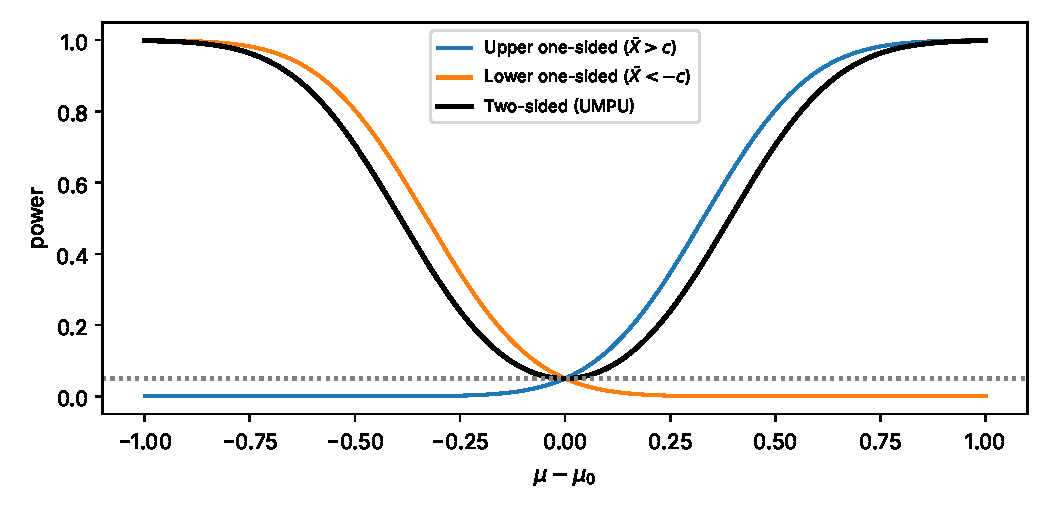
\includegraphics[width=0.8\textwidth]{figures/iki_tarafli.pdf}
\caption{Power functions of three tests for $H_1:\mu\neq\mu_0$ ($n=25$, $\sigma=1$). Each one-sided test is more powerful than the two-sided test in its own direction, but in the other direction its power falls even below $\alpha$ (it is biased). No test is most powerful at every $\mu\neq\mu_0$; the two-sided test is most powerful among unbiased tests.}
\end{figure}

\subsection{Uniform: MLR and the Power of the UMP Test}

\pycode{code/ch14/c14_3_uniform_mlr_ump_power.py}
\begin{lstlisting}[style=output]
theta=0.9 | rejection rate=0.0000 | theory=0.0000
theta=1.0 | rejection rate=0.0505 | theory=0.0500
theta=1.1 | rejection rate=0.5587 | theory=0.5568
theta=1.3 | rejection rate=0.8836 | theory=0.8835
\end{lstlisting}

\section{Comments and Notes}

\begin{remark}[The Rarity of UMP Tests]
UMP\index{uniformly most powerful ump test@uniformly most powerful (UMP) test} tests exist essentially in one-parameter families with MLR\index{monotone likelihood ratio mlr@monotone likelihood ratio (MLR)} and for one-sided hypotheses. In multiparameter problems (e.g.\ testing a normal mean with $\sigma$ unknown) the presence of a nuisance parameter\index{nuisance parameter@nuisance parameter} usually rules out a UMP test; one then uses either (a) optimality under additional constraints such as unbiasedness or invariance (UMPU\index{umpu test@UMPU test}, UMPI; the $t$-test is optimal in this sense) or (b) the general likelihood ratio\index{likelihood ratio@likelihood ratio} test\index{likelihood ratio test lrt@likelihood ratio test (LRT)} of Chapter~\ref{ch:lrt}.
\end{remark}

\begin{remark}[One-Sided or Two-Sided?]
A one-sided test is more powerful when its direction is scientifically justified in advance (before seeing the data). Choosing the direction after looking at the data effectively raises the type I\index{type i and type ii errors@type I and type II errors} error to $2\alpha$. For this reason regulators (e.g.\ for clinical trials) usually require two-sided tests or one-sided tests at level $\alpha/2$.
\end{remark}

% --- CHAPTER SUMMARY ---
\section{Chapter Summary}
\begin{summary}
\begin{itemize}
  \item For composite alternatives, a test that is most powerful simultaneously for all parameter values is called UMP. Such a test exists only in special structures.
  \item A monotone likelihood ratio (Definition~\ref{def:mlr}) provides this structure. In the exponential family there is MLR if $w(\theta)$ is monotone (Proposition~\ref{prop:ustel-mlr}).
  \item The Karlin--Rubin theorem (Theorem~\ref{thm:karlin-rubin}): in MLR families the test ``$T>c$'' is UMP for one-sided hypotheses.
  \item There is no UMP test in the two-sided problem (Proposition~\ref{prop:iki-tarafli}). Adding the constraint of unbiasedness yields a UMPU test in the exponential family (Theorem~\ref{thm:umpu}).
\end{itemize}
\end{summary}
% --- END OF CHAPTER SUMMARY ---

\paragraph{Further reading.} \cite[Section~8.3]{casella}, \cite[Chapters~3--4]{lehmann-romano}.

\section{Exercises}

\begin{exercise}\label{exr:14-1}
$X_i\iid\text{Poisson}(\lambda)$, $H_0:\lambda\le1$, $H_1:\lambda>1$, $n=20$, $\alpha=0.05$. Construct the UMP randomised test and plot its power function on the interval $\lambda\in[0.5,\,2]$.
\hfill\hyperref[coz:14-1]{\footnotesize$\rightarrow$\,Solution}
\end{exercise}

\begin{exercise}\label{exr:14-2}
For $X_i\iid\Normal(0,\sigma^2)$, find the UMP test against $H_0:\sigma\le\sigma_0$. Show numerically that for $H_0:\sigma=\sigma_0$, $H_1:\sigma\ne\sigma_0$ the equal-tailed chi-square test is \emph{biased}.
\hfill\hyperref[coz:14-2]{\footnotesize$\rightarrow$\,Solution}
\end{exercise}

\begin{exercise}\label{exr:14-3}
Show that the logistic location family $f(x;\theta)=\frac{e^{-(x-\theta)}}{(1+e^{-(x-\theta)})^2}$ has MLR in $x$ (a single observation). Discuss why for $n>1$ there is no MLR in $\sum X_i$, so that Karlin--Rubin cannot be applied directly.
\hfill\hyperref[coz:14-3]{\footnotesize$\rightarrow$\,Solution}
\end{exercise}

\begin{exercise}\label{exr:14-4}
Using Step~2 of the proof of Theorem~\ref{thm:karlin-rubin}, show that in a family with MLR the $p$-value is $p(\x)=\P_{\theta_0}(T\ge T(\x))$ and that, for the composite $H_0:\theta\le\theta_0$, the supremum is attained at $\theta_0$.
\hfill\hyperref[coz:14-4]{\footnotesize$\rightarrow$\,Solution}
\end{exercise}

\chapterlinks{14}

\end{document}
